\documentclass{article}
\usepackage[utf8]{inputenc}
\usepackage[T1]{fontenc}
\usepackage{lmodern}
\usepackage{amsmath,amssymb,amsthm}
\usepackage{graphicx}
\usepackage{booktabs}
\usepackage{longtable}
\usepackage{array}
\usepackage{enumitem}
\usepackage{hyperref}
\usepackage{cleveref}
\usepackage{float}
\usepackage{subcaption}
\usepackage{caption}
\usepackage{geometry}
\usepackage{color}
\usepackage{xcolor}
\usepackage{listings}
\usepackage{algorithm}
\usepackage{algorithmic}
\usepackage{chemfig}
\usepackage{siunitx}
\usepackage{natbib}
\usepackage{biblatex}
\usepackage{filecontents}
\usepackage{tikz}
\usetikzlibrary{shapes,arrows,positioning,chains,fit,decorations.pathreplacing}
\usepackage{pgfplots}
\pgfplotsset{compat=1.18}
\usepackage{forest}
\usepackage{csquotes}
\usepackage{lipsum}

\title{Comprehensive \LaTeX{} Example}
\author{Mathew Writer\thanks{Corresponding author}}
\date{\today}

\begin{document}

\maketitle

\begin{abstract}
This document demonstrates comprehensive \LaTeX{} features including advanced mathematical typesetting, figures, tables, algorithms, code listings, cross-referencing, bibliographies, and more.
\end{abstract}

\tableofcontents
\newpage

\section{Introduction}
\LaTeX{} is a high-quality typesetting system designed for technical and scientific documentation. It is the de facto standard for communication and publication of scientific documents.

\section{Document Structure}
\subsection{Sectioning Commands}
\LaTeX{} provides hierarchical sectioning: \verb|\part|, \verb|\chapter| (in book/report classes), \verb|\section|, \verb|\subsection|, \verb|\subsubsection|, \verb|\paragraph|, \verb|\subparagraph|.

\subsection{Cross-referencing}
Using \verb|\label| and \verb|\ref|, we can refer to sections (\cref{sec:math}), figures (\cref{fig:example}), tables (\cref{tab:example}), and equations (\cref{eq:euler}).

\section{Mathematics}
\LaTeX{} excels at typesetting mathematics.

\subsection{Inline Mathematics}
Inline math: $E=mc^2$, $\displaystyle \sum_{n=1}^{\infty} \frac{1}{n^2} = \frac{\pi^2}{6}$, and $\int_{-\infty}^{\infty} e^{-x^2} dx = \sqrt{\pi}$.

\subsection{Displayed Mathematics}
\begin{equation}
\label{eq:euler}
e^{i\pi} + 1 = 0
\end{equation}

\begin{align}
\label{eq:heat}
\frac{\partial u}{\partial t} - \alpha \nabla^2 u &= 0 \\
\nabla \cdot \mathbf{E} &= \frac{\rho}{\epsilon_0} \\
\nabla \times \mathbf{B} - \mu_0 \epsilon_0 \frac{\partial \mathbf{E}}{\partial t} &= \mu_0 \mathbf{J}
\end{align}

\subsection{Matrices and Arrays}
\[
A = \begin{pmatrix}
a_{11} & a_{12} & \cdots & a_{1n} \\
a_{21} & a_{22} & \cdots & a_{2n} \\
\vdots & \vdots & \ddots & \vdots \\
a_{m1} & a_{m2} & \cdots & a_{mn}
\end{pmatrix}
\]

\[
\det(A) = \left|
\begin{array}{ccc}
a & b & c \\
d & e & f \\
g & h & i
\end{array}
\right| = aei + bfg + cdh - ceg - bdi - afh
\]

\subsection{Theorems and Proofs}
\begin{theorem}[Pythagorean Theorem]
In a right triangle, the square of the hypotenuse is equal to the sum of the squares of the other two sides.
\end{theorem}

\begin{proof}
Let the triangle have sides $a$, $b$, and hypotenuse $c$. By constructing squares on each side and using area arguments, we show $a^2 + b^2 = c^2$.
\end{proof}

\section{Figures and Graphics}
\subsection{Including Images}
\begin{figure}[H]
    \centering
    % Placeholder for actual image
    \fbox{\parbox{0.8\linewidth}{\centering Image Placeholder \\[10pt] (Replace with actual image)}}
    \caption{Example figure placeholder}
    \label{fig:example}
\end{figure}

\subsection{TikZ Graphics}
\begin{figure}[H]
    \centering
    \begin{tikzpicture}
        \draw[->] (0,0) -- (4,0) node[right] {$x$};
        \draw[->] (0,0) -- (0,3) node[above] {$y$};
        \draw[scale=0.5,domain=-2:2,smooth,variable=\x,blue] plot ({\x},{\x*\x});
        \node[above right] at (2,4) {$y = x^2$};
    \end{tikzpicture}
    \caption{Simple TikZ plot}
    \label{fig:tikz}
\end{figure}

\subsection{Plots with PGFPlots}
\begin{figure}[H]
    \centering
    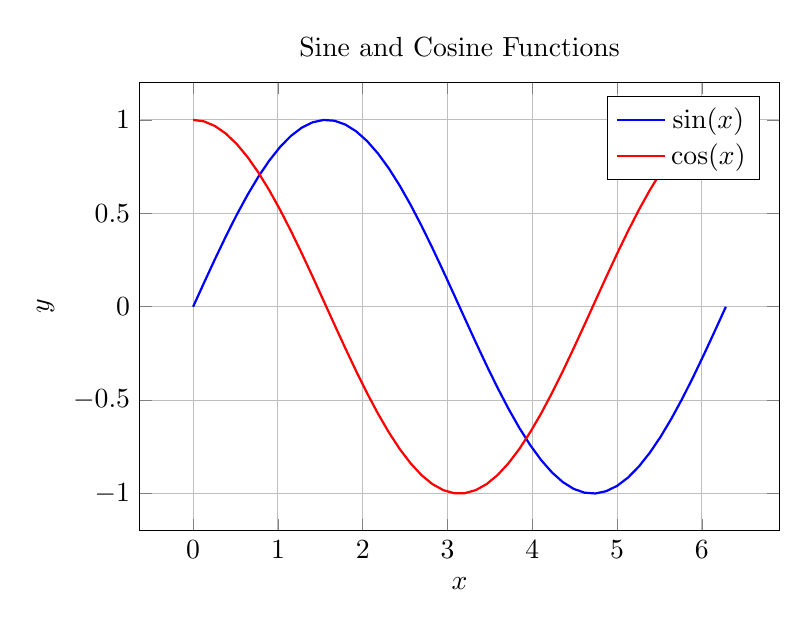
\begin{tikzpicture}
        \begin{axis}[
            title={Sine and Cosine Functions},
            xlabel={$x$},
            ylabel={$y$},
            legend pos=north east,
            grid=major,
            width=0.8\textwidth,
            height=0.6\textwidth
        ]
        \addplot[blue, thick, domain=0:2*pi,samples=50] {sin(deg(x))};
        \addlegendentry{$\sin(x)$}
        \addplot[red, thick, domain=0:2*pi,samples=50] {cos(deg(x))};
        \addlegendentry{$\cos(x)$}
        \end{axis}
    \end{tikzpicture}
    \caption{PGFPlots example}
    \label{fig:pgfplots}
\end{figure}

\section{Tables}
\begin{table}[H]
    \centering
    \caption{Example table with booktabs}
    \label{tab:example}
    \begin{tabular}{@{}lcc@{}}
        \toprule
        \textbf{Method} & \textbf{Accuracy (\%)} & \textbf{Time (s)} \\
        \midrule
        Method A & 95.2 & 1.2 \\
        Method B & 92.8 & 0.8 \\
        Method C & 97.5 & 2.1 \\
        \bottomrule
    \end{tabular}
\end{table}

\subsection{Long Tables}
\begin{longtable}{@{}lll@{}}
    \caption{Long table example}\\
    \toprule
    \textbf{Parameter} & \textbf{Value} & \textbf{Description} \\
    \midrule
    \endfirsthead
    \multicolumn{3}{c}{{\tablename\ \thetable{} -- continued from previous page}} \\
    \toprule
    \textbf{Parameter} & \textbf{Value} & \textbf{Description} \\
    \midrule
    \endhead
    \midrule
    \multicolumn{3}{r}{{Continued on next page}} \\
    \endfoot
    \bottomrule
    \endlastfoot
    Temperature & \SI{300}{\kelvin} & Ambient temperature \\
    Pressure & \SI{1}{\atmosphere} & Atmospheric pressure \\
    Volume & \SI{22.4}{\liter\per\mole} & Molar volume \\
    Gas Constant & \SI{8.314}{\joule\per\mole\per\kelvin} & Universal gas constant \\
    Avogadro's Number & \num{6.022e23} & \si{\per\mole} \\
    \addlinespace
    Speed of Light & \SI{2.998e8}{\meter\per\second} & Vacuum speed of light \\
    Planck's Constant & \SI{6.626e-34}{\joule\second} & Quantum of action \\
    Electron Charge & \SI{1.602e-19}{\coulomb} & Elementary charge \\
    Electron Mass & \SI{9.109e-31}{\kilogram} & Mass of electron \\
    Bohr Radius & \SI{0.529}{\angstrom} & Bohr radius \\
\end{longtable}

\section{Code Listings}
Using the \texttt{listings} package:

\begin{lstlisting}[language=Python, caption={Python function to compute factorial}, label={lst:factorial}]
def factorial(n):
    """Return the factorial of n, an exact integer >= 0."""
    if n < 0:
        raise ValueError("n must be >= 0")
    if n == 0:
        return 1
    else:
        return n * factorial(n-1)
\end{lstlisting}

With syntax highlighting for other languages:

\begin{lstlisting}[language=C++, caption={Hello World in C++}, label={lst:hello}]
#include <iostream>

int main() {
    std::cout << "Hello, World!" << std::endl;
    return 0;
}
\end{lstlisting}

\section{Algorithms}
Using the \texttt{algorithm} and \texttt{algorithmic} packages:

\begin{algorithm}
\caption{Euclidean algorithm for GCD}
\label{alg:euclid}
\begin{algorithmic}
\REQUIRE $a,b \geq 0$
\ENSURE $g = \gcd(a,b)$
\STATE $r \gets a \bmod b$
\WHILE $r \neq 0$
\STATE $a \gets b$
\STATE $b \gets r$
\STATE $r \gets a \bmod b$
\ENDWHILE
\RETURN $b$
\end{algorithmic}
\end{algorithm}

\section{Chemistry}
Using \texttt{chemfig} for chemical structures:

\begin{figure}[H]
    \centering
    \chemfig{C(-[2]H)(-[6]H)-C(-[2]H)(-[6]H)=C(-[2]H)(-[6]H)-C(-[2]H)(-[6]H)}
    \caption{Butane structure}
    \label{fig:butane}
\end{figure}

Or using \texttt{mhchem} (if loaded): $\ce{CO2 + C -> 2 CO}$

\section{Bibliography}
We can cite sources using \texttt{natbib} or \texttt{biblatex}. For demonstration, we'll create a simple bibliography using the \texttt{thebibliography} environment.

\begin{thebibliography}{9}
\bibitem{latexcompanion}
Michel Goossens, Frank Mittelbach, and Alexander Samarin.
\textit{The \LaTeX{} Companion}.
Addison-Wesley, Reading, Massachusetts, 1993.

\bibitem{knuth:1984}
Donald E. Knuth.
\textit{The \TeX{}book}.
Addison-Wesley Professional, 1984.

\bibitem{lamport94}
Leslie Lamport.
\textit{\LaTeX:} A Document Preparation System.
Addison-Wesley, Reading, Massachusetts, second edition, 1994.
\end{thebibliography}

See \cite{latexcompanion} for more information.

\section{Conclusion}
\LaTeX{} provides extensive features for creating professional documents. This sample showcases only a fraction of its capabilities, including mathematical typesetting, figures, tables, code listings, algorithms, and bibliographies.

\end{document}